\section{More About Normal Distribution}

\subsection{Normal Distribution}

\begin{frame}{Normal Distribution}

\justifying
\structb{Definition.} A continuous random variable $(X, f_{\mu, \sigma^2})$ has the \highlightg{normal distribution} with mean $\mu \in \R$ and variance $\sigma^2, \sigma > 0$ if the probability density function is given by
\begin{align*}
f_{\mu, \sigma^2} = \frac{1}{\sqrt{2\pi \sigma^2}} \exp\left[-\frac{1}{2}\left(\frac{x-\mu}{\sigma} \right)^2 \right], \qquad x\in \R.
\end{align*}

\end{frame}

\begin{frame}{Normal Distribution}

\justifying
\structb{Mean, variance and M.G.F.} 
\begin{itemize}
\justifying
\item \underline{Mean}. 
\begin{align*}
\U{E}[X] = \mu.
\end{align*}
\item \underline{Variance}.
\begin{align*}
\U{Var}[X] = \sigma^2.
\end{align*}
\item \underline{M.G.F.}
\begin{align*}
m_X: \R \rightarrow \R, \qquad m_X(t) = \exp\left(\mu t + \frac{1}{2}\sigma^2t^2 \right).
\end{align*}
\end{itemize}

\end{frame}

\begin{frame}{Normal Distribution}

\structb{Verifying M.G.F.}
\begin{align*}
m_X(t) & = \U{E}\left[e^{tX} \right] = \int_{-\infty}^{\infty} \frac{e^{tx}}{\sqrt{2\pi }\sigma} e^{-((x-\mu)/\sigma)^2/2}\U{d}x \\
& = \frac{1}{\sqrt{2\pi}\sigma} \int_{-\infty}^{\infty} e^{\mu t + \sigma^2 t^2/2} \cdot e^{-\frac{(x-(\mu + \sigma^2 t))^2}{2\sigma^2}} \U{d}x \\
& = e^{\mu t + \sigma^2 t^2/2} \underbrace{\frac{1}{\sqrt{2\pi}\sigma} \int_{-\infty}^{\infty} e^{-\frac{(x-(\mu + \sigma^2 t))^2}{2\sigma^2}} \U{d}x}_{= 1} \\
& = e^{\mu t + \sigma^2 t^2/2}.
\end{align*}

\end{frame}

\begin{frame}{Normal Distribution}

\structb{Some takeaway from this proof.}
\begin{itemize}
	\justifying
	\item To verify that
	\begin{align*}
	I := \int_{-\infty}^{\infty} e^{-\frac{(x-b)^2}{a^2}}\U{d}x = a\sqrt{\pi},
	\end{align*}
	we use
	\begin{align*}
	I^2 = \left(\int_{-\infty}^{\infty} e^{-\frac{(x-a)^2}{b^2}}\U{d}x \right)^2 = \int_{-\infty}^{\infty} e^{-\frac{(x-a)^2}{b^2}}\cdot e^{-\frac{(y-a)^2}{b^2}} \U{d}x\U{d}y.
	\end{align*}
	Using parametrization $x = ar\cos\theta + b, y = ar\sin\theta + b$, we have
	\begin{align*}
	I^2 & = \int_0^{\infty}\int_{0}^{2\pi} e^{-r^2} \cdot a^2r\U{d}\theta \U{d}r \\
	& = a^2\pi \int_{0}^{\infty} 2r e^{-r^2}\U{d}r = -a^2\pi e^{-r^2}\bigg|_0^{\infty} = a^2\pi.
	\end{align*}
\end{itemize}

\end{frame}


\begin{frame}{Normal Distribution}

\structb{Some takeaway from this proof.}
\begin{itemize}
	\justifying
	\item Useful results from normalizing constant of distributions.
	\begin{enumerate}[(i).]
		\item \underline{Normal}.
		\begin{align*}
		\int_{-\infty}^{\infty} e^{-\frac{(x-\mu)^2}{2\sigma^2}}\U{d}x = \sqrt{2\pi}\sigma.
		\end{align*}
		\item \underline{Gamma}.
		\begin{align*}
		\int_0^{\infty} x^{\alpha-1} e^{-\beta x}\U{d}x = \frac{\Gamma(\alpha)}{\beta^{\alpha}}.
		\end{align*}
	\end{enumerate}
\end{itemize}

\end{frame}


\begin{frame}{Transformation of Random Variables}

\begin{itemize}
	\justifying
	\item \structb{Discrete random variables}. Let $X$ be a discrete random variable with probability density function $f_X$, the the probability density function $f_Y$ for $Y = \varphi(X)$ is given by
	\begin{align*}
	f_Y(y) = \sum_{x\in \varphi^{-1}(y)} f_X(x), \qquad \U{for\ } y\in \U{ran}\ \varphi,
	\end{align*}
	and 0 otherwise.\\
	\structb{Example 1}. Let $X$ be a uniform random variable on $\{-n, -n+1, \ldots, n-1, n\}$. Then $Y = |X|$ has probability density function
	\begin{align*}
	f_Y(y) = \left\{
	\begin{array}{ll}
	\dfrac{1}{2n+1} & x = 0, \\
	\dfrac{2}{2n+1} & x\neq 0.
	\end{array}
	\right.
	\end{align*}
\end{itemize}


\end{frame}


\begin{frame}{Transformation of Random Variables}


\begin{itemize}
\justifying
\item \structb{Continuous random variables}. Let $X$ be a continuous random variable with density $f_X$. Let $Y = \varphi\circ X$, where $\varphi: \R\rightarrow \R$ is strictly monotonic and differentiable. The density for $Y$ is then given by
\begin{align*}
f_Y(y) = f_X(\varphi^{-1}(y))\cdot \left|\frac{\U{d}\varphi^{-1}(y)}{\U{d}y} \right|, \qquad \U{for\ } y\in \U{ran\ }\varphi
\end{align*}
and 
\begin{align*}
f_Y(y) = 0, \qquad \U{for\ } y\notin \U{ran\ } \varphi.
\end{align*}
\uncover<2>{
	For multivariate random variables, $\mathbf{Y} = \varphi\circ \mathbf{X}$, we have
	\begin{align*}
	f_{\mathbf{Y}}(y) = f_{\mathbf{X}}\circ \varphi^{-1}(y) \cdot |\det\ D\varphi^{-1}(y)|,
	\end{align*}
	where $D\varphi^{-1}$ is the Jacobian of $\varphi^{-1}$.
}
\end{itemize}


\end{frame}



\begin{frame}{Sum of Normal Distributions}

\structb{Theorem.} If the random variables $X_1, \ldots, X_k$ are independent and if $X_i$ has the normal distribution with mean $\mu_i$ and variances $\sigma_i^2$, where $i = 1, \ldots, k$, then the sum 
\begin{align*}
X = X_1 + \cdots + X_k
\end{align*}
follows the normal distribution with
\begin{align*}
\mu = \mu_1 + \cdots + \mu_k, \qquad \sigma^2 = \sigma_1^2 + \cdots + \sigma_k^2.
\end{align*}
\uncover<2>{
	\structb{Proof (sketch).} Using M.G.F., we have
	\begin{align*}
	m_X(t) & = \prod_{i=1}^k m_{X_i}(t) = \prod_{i=1}^k \exp\left(\mu_i t + \frac{1}{2}\sigma_i^2 t^2\right) \\
	& = \exp\left[\left(\sum_{i=1}^k \mu_i \right)t + \frac{1}{2}\left(\sum_{i=1}^k \sigma_i^2 \right)t^2 \right], \qquad t\in \R.
	\end{align*}
}

\end{frame}


\begin{frame}{Quotient of Normal Distributions}

\justifying
\structb{Theorem.} Suppose that random variables $X$ and $Y$ are independent and that each has the standard normal distribution. Then $U = X/Y$ has the \emph{Cauchy distribution} with probability density function given by
\begin{align*}
f_U(u) = \frac{1}{\pi(1+u^2)}, \qquad u\in \R.
\end{align*}\\
\only<2>{
	\justifying
	\structb{Proof (sketch).} Let $V = Y$, excluding $Y = 0$, the transformation from $(X, Y)$ to $(U, V)$ is one-to-one. Then $X = UV, Y = V$ and
	\begin{align*}
	J = \det\begin{pmatrix}
	\dfrac{\partial x}{\partial u} & \dfrac{\partial x}{\partial v} \\
	\dfrac{\partial y}{\partial u} & \dfrac{\partial y}{\partial v}
	\end{pmatrix} = v.
	\end{align*}
}
\uncover<3>{
	\justifying
	\structb{Proof (sketch, continued).} Then the joint density function is given by
	\begin{align*}
	f_{UV}(u, v) = f_{XY}(uv, v)|v| = \frac{|v|}{2\pi} \exp\left(-\frac{1}{2}(u^2+1)v^2 \right).
	\end{align*}
	Then the marginal of $U$ is calculated as
	\begin{align*}
	f_U(u) & = \int_{-\infty}^{\infty} f_{UV}(u, v) \U{d}v = \frac{1}{\pi(u^2+1)}, \quad u\in\R.
	\end{align*}
}



\end{frame}


\begin{frame}{Standardizing Normal Distribution}

\justifying
Suppose $X\sim \U{Normal}(\mu, \sigma^2)$. Then 
\begin{align*}
Z = \frac{X-\mu}{\sigma} \sim \U{Normal}(0, 1),
\end{align*}
where the normal distribution with mean $\mu$ and variance $\sigma^2$ is the \highlightg{standard normal distribution}. Furthermore, the cumulative distri-\\bution function of $X$ is given by
\begin{align*}
F(x) = \Phi\left(\frac{x-\mu}{\sigma} \right), \quad F^{-1}(p) = \mu + \sigma \Phi^{-1}(p),
\end{align*}
where $\Phi$ is the cumulative distribution function for the standard normal distribution function.

\end{frame}

\subsection{Applications of Normal Distribution}

\begin{frame}{Common Applications of Normal Distribution}

\justifying
Suppose a random variable $X$ follows normal distribution $N(\mu, \sigma)$, where $\mu$ and $\sigma$ are known. At current stage, applications usually include the following.
\begin{enumerate}
	\justifying
	\item Given some value $x_0$, find the probability of $P[X \leq x_0]$ or $P[X\geq x_0]$.
	\begin{enumerate}[(a).]
		\justifying
		\item Standardize $X$ as $Z = (X - \mu) / \sigma$, find $z_0$.
		\item Find $P[X \leq x_0] = P[Z\leq z_0], P[X\geq x_0] = 1 - P[Z\geq z_0]$.
	\end{enumerate}
	\item Given some probability $p$, find the corresponding $x_0$ such that $P[X\leq x_0] = p$ or $P[X\geq x_0] = p$.
	\begin{enumerate}[(a).]
		\justifying
		\item Find $z_0$ from table such that $P[Z\leq z_0] = p$ or $P[Z\leq z_0] = 1 - p$.
		\item Calculate $x_0 = \sigma z_0 + \mu$.
	\end{enumerate}
	\item ``Three-sigma'' rule.
	\begin{align*}
	P[-3\sigma < X-\mu < 2\sigma] = 0.997.
	\end{align*}
\end{enumerate}

\end{frame}


\begin{frame}{The Chebyshev's Inequality}

\justifying
\structb{Theorem.} Let $X$ be a random variable, then for $k\in \N\setminus\{0\}$ and $c > 0$,
\begin{align*}
P[|X| \geq c] \leq \frac{\U{E}[|X|^k]}{c^k}.
\end{align*}
As another version of this inequality, suppose $X$ has mean $\mu$ and standard deviation $\sigma$, and let $m > 0$,
\begin{align*}
P[|X - \mu| \geq m\sigma] \leq \frac{1}{m^2},
\end{align*}
or equivalently,
\begin{align*}
P[-m\sigma < X - \mu < m\sigma] \geq 1 - \frac{1}{m^2}.
\end{align*}
\highlightr{Note.} This yields another (looser) version of $\sigma, 2\sigma, 3\sigma$ rule for normal distribution.

\end{frame}


\begin{frame}{Application of Chebyshev's Inequality}

\justifying
\structb{Weak Law of Large Numbers.} Let $X_1, X_2, \ldots$ be a sequence of i.i.d. random variables with mean $\mu$ and variance $\sigma^2$. Then for any $\varepsilon > 0$,
\begin{align*}
P\left[\left|\frac{X_1 + \ldots + X_n}{n} - \mu \right| \geq \varepsilon \right] \xrightarrow{n\rightarrow \infty} 0.
\end{align*}
~\\
\only<2>{
	\justifying
	\structb{Law of Large Numbers.} Let $A$ be a random outcome (random event) of an experiment that can be repeated without the outcome influencing subsequent repetitions. Then the probability $P[A]$ of this event occurring may be approximated by 
	\begin{align*}
	P[A] \approx \frac{\U{number\ of\ times\ } A \U{\ occurs}}{\U{number\ of\ times\ experiment\ is\ perfomred}}.
	\end{align*}
	\highlightr{Note.} Approximate mean $\mu = p = P[A]$ of Bernoulli distribution.\\
}
\only<3>{
	\justifying
	\structb{Proof.} Using properties of expectation and variance,
	\begin{align*}
	\U{E}\left[\frac{X_1 + \cdots + X_n}{n} - \mu \right] & = \frac{\U{E}[X_1] + \cdots + \U{E}[X_n]}{n} - \U{E}[\mu] = 0, \\
	\U{Var}\left[\frac{X_1 + \cdots + X_n}{n} - \mu \right] & = \frac{\U{Var}[X_1] + \cdots + \U{Var}[X_n]}{n^2} + \U{Var}[\mu] = \frac{\sigma^2}{n}, \\
	& \Rightarrow \quad \U{E}\left[\left(\frac{X_1 + \cdots + X_n}{n} - \mu \right)^2 \right] = \frac{\sigma^2}{n}.
	\end{align*}
}
\uncover<4>{
	\justifying
	Applying the Chebyshev's inequality with $k = 2$ to 
	\begin{align*}
	X = \dfrac{X_1 + \cdots + X_n}{n} - \mu,
	\end{align*}
	we have
	\begin{align*}
	P\left[\left|\frac{X_1 + \ldots + X_n}{n} - \mu \right| \geq \varepsilon \right] \leq \frac{\sigma^2}{n\varepsilon^2} \xrightarrow{n\rightarrow \infty} 0.
	\end{align*}
}

\end{frame}



\begin{frame}{Normal Approximation of Binomial Distribution}

\justifying
Suppose $S_n$ is the number of successes in a sequence of $n$ i.i.d. Bernoulli trials with probability of success $0 < p < 1$.
\begin{itemize}
	\justifying
	\item It satisfies that
	\begin{align*}
	\lim_{n\rightarrow \infty} P\left[a < \frac{X-np}{\sqrt{np(1-p)}} \leq b \right] = \frac{1}{2\pi} \int_a^b e^{-x^2/2} \U{d}x.
	\end{align*}
	\item For $y = 0, \ldots, n$,
	\begin{align*}
	P[X\leq y] = \sum_{x=0}^y \binom{n}{x} p^x(1-p)^{n-x} \approx \Phi\left(\frac{y\red{+1/2}-np}{\sqrt{np(1-p)}} \right),
	\end{align*}
	where we require that
	\begin{align*}
	np > 5 \quad \U{if\ } p\leq \frac{1}{2} \qquad \U{or}\qquad n(1-p) > 5 \quad \U{if\ } p > \frac{1}{2}.
	\end{align*}
\end{itemize}

\end{frame}



\section{Multivariate Random Variables}

\subsection{Discrete Multivariate Random Variables}

\begin{frame}{Discrete Multivariate Random Variables}

\justifying
\structb{Definition.} Let $S$ be a sample space and $\Omega$ a countable subset of $\R^n$. A \highlightg{discrete multivariate random variable} is a map
\begin{align*}
\mathbf{X}: S\rightarrow \Omega
\end{align*}
together with a function $f_{\mathbf{X}}: \Omega\rightarrow\R$ with the properties that
\begin{enumerate}[(i).]
	\item $f_{\mathbf{X}}(x) \geq 0$ for all $x = (x_1, \ldots, x_n)\in \Omega$ and
	\item $\displaystyle \sum_{x\in \Omega} f_{\mathbf{X}}(x) = 1$,
\end{enumerate}
where $f_{\mathbf{X}}$ is the \highlightg{joint density function} of the random variable $\mathbf{X}$.

\end{frame}

\begin{frame}{Discrete Multivariate Random Variables}

\justifying
\structb{Definition.} 
\begin{itemize}
	\item \highlightg{Marginal density} $f_{X_k}$ for $X_k, k = 1, \ldots, n$:
	\begin{align*}
	f_{X_k}(x_k) = \sum_{x_1, \ldots, x_{k-1}, x_{k+1}, \ldots, x_n} f_{\mathbf{X}}(x_1, \ldots, x_n).
	\end{align*}
	\item \highlightg{Independent} multivariate random variables:
	\begin{align*}
	f_{\mathbf{X}}(x_1, \ldots, x_n) = f_{X_1}(x_1)\cdots f_{X_n}(x_n).
	\end{align*}
	\item \highlightg{Conditional density} of $X_1$ conditioned on $X_2$:
	\begin{align*}
	f_{X_1|X_2}(x_1) := \frac{f_{X_1X_2}(x_1, x_2)}{f_{X_2}(x_2)} \qquad \U{whenever\ } f_{X_2}(x_2) > 0.
	\end{align*}
\end{itemize}

\end{frame}


\subsection{Continuous Multivariate Random Variables}


\begin{frame}{Continuous Multivariate Random Variables}

\justifying
\structb{Definition.} Let $S$ be a sample space. A \highlightg{continuous multivariate random variable} is a map
\begin{align*}
\mathbf{X}: S\rightarrow \R^n
\end{align*}
together with a function $f_{\mathbf{X}}: \R^n\rightarrow\R$ with the properties that
\begin{enumerate}[(i).]
	\item $f_{\mathbf{X}}(x) \geq 0$ for all $x = (x_1, \ldots, x_n)\in \R^n$ and
	\item $\displaystyle \int_{\R^n} f_{\mathbf{X}}(x) = 1$,
\end{enumerate}
where $f_{\mathbf{X}}$ is the \highlightg{joint density function} of the random variable $\mathbf{X}$.

\end{frame}

\begin{frame}{Continuous Multivariate Random Variables}

\justifying
\structb{Definition.} 
\begin{itemize}
\item \highlightg{Marginal density} $f_{X_k}$ for $X_k, k = 1, \ldots, n$:
\begin{align*}
f_{X_k}(x_k) = \int_{\R^{n-1}} f_{\mathbf{X}}(x_1, \ldots, x_n) \U{d}x_1\ldots \U{d}x_{k-1}\U{x_{k+1}}\ldots \U{d}x_n.
\end{align*}
\item \highlightg{Independent} multivariate random variables:
\begin{align*}
f_{\mathbf{X}}(x_1, \ldots, x_n) = f_{X_1}(x_1)\cdots f_{X_n}(x_n).
\end{align*}
\item \highlightg{Conditional density} of $X_1$ conditioned on $X_2$:
\begin{align*}
f_{X_1|X_2}(x_1) := \frac{f_{X_1X_2}(x_1, x_2)}{f_{X_2}(x_2)} \qquad \U{whenever\ } f_{X_2}(x_2) > 0.
\end{align*}
\end{itemize}

\end{frame}


\begin{frame}{Continuous Multivariate Random Variables}

\justifying
\structb{Visualization.} Joint probability density function $f_{XY}(x, y)$ (left) and conditional density function $f_{X|Y}(x|y_0)$ (right).\\
~\\
\begin{minipage}{0.5\linewidth}
	\centering
	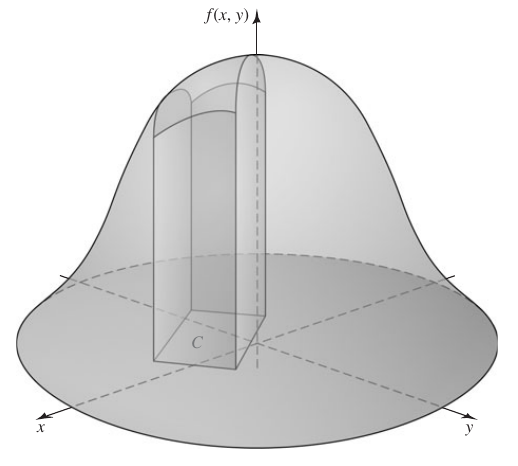
\includegraphics[width=5cm]{./images/rc3fig1.png}
\end{minipage}
\begin{minipage}{0.5\linewidth}
	\centering
	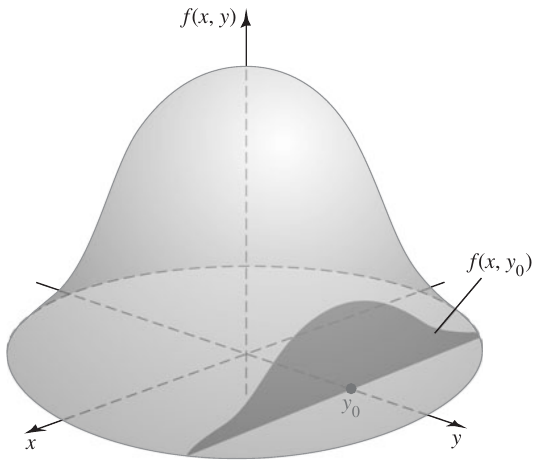
\includegraphics[width=5cm]{./images/rc3fig2.png}
\end{minipage}

\end{frame}


\begin{frame}{Continuous Multivariate Random Variables}

\justifying
\structb{Q.} How to determine the joint probability density function and cumulative distribution function of a single variable from a joint cumulative distribution function? \\
\uncover<2>{
	~\\
	\justifying
	\structb{C.D.F.} For continuous random variables $X_1, \ldots, X_n$, the joint cumula-tive distribution function is then given by
	\begin{align*}
	P[X_1 \leq a_1, \ldots, X_n\leq a_n] = \int_{-\infty}^{a_1}\cdots \int_{-\infty}^{a_n} f_{\mathbf{X}}(x) \U{d}x_1\ldots \U{d}x_n.
	\end{align*}
}

\end{frame}

\begin{frame}{Continuous Multivariate Random Variables}

\justifying
\structb{Example 2.} Suppose $X$ and $Y$ are random variables that take values in the intervals $0\leq X\leq 2$ and $0\leq Y\leq 2$. Suppose the joint cumulative distribution function for $x\in [0, 2], y\in [0, 2]$ is given by
\begin{align*}
F(x, y) = \frac{1}{16}xy(x + y).
\end{align*}
What are the joint density function and cumulative distribution of $X$? \\
\only<2>{
	\justifying
	\structb{Solution (i).} For $x \in [0, 2], y\in [0, 2]$,
	\begin{align*}
	f(x, y) = \frac{\partial^2 F(x, y)}{\partial x\partial y} = \frac{1}{8}(x + y),
	\end{align*}
	and thus
	\begin{align*}
	f_{XY}(x, y) = \left\{
	\begin{array}{ll}
	\dfrac{1}{8}(x+y) & 0\leq x\leq 2, 0 \leq y\leq 2 \\
	0 & \U{otherwise}.
	\end{array}
	\right.
	\end{align*}
}
\uncover<3>{
	\justifying
	\structb{Solution (ii).} Since for $y > 2$, $F(x, y) = F(x, 2)$, then by letting $y\rightarrow\infty$, we obtain
	\begin{align*}
	F_X(x) = \left\{
	\begin{array}{ll}
	0 & x < 0, \\
	\dfrac{1}{8}x(x+2) & 0\leq x\leq 2, \\
	1 & x > 2.
	\end{array}
	\right.
	\end{align*}
}

\end{frame}



\subsection{Expectation and Variance}

\begin{frame}{Expectation}

\begin{itemize}
	\item \underline{Discrete}.
	\begin{align*}
	\U{E}[X_k] = \sum_{x_k}x_kf_{X_k}(x_k) = \sum_{x\in \Omega} x_k f_{\mathbf{X}}(x),
	\end{align*}
	and for continuous function $\varphi: \R^n\rightarrow \R$,
	\begin{align*}
	\U{E}[\varphi\circ \mathbf{X}] = \sum_{x\in \Omega} \varphi(x)f_{\mathbf{X}}(x).
	\end{align*}
	\item \underline{Continuous}.
	\begin{align*}
	\U{E}[X_k] = \int_{\R} x_k f_{X_k}(x_k) \U{d}x_k = \int_{\R^n} x_kf_{\mathbf{X}}(x)\U{d}x,
	\end{align*}
	and for continuous function $\varphi: \R^n\rightarrow \R$,
	\begin{align*}
	\U{E}[\varphi\circ \mathbf{X}] = \int_{\R^n} \varphi(x)f_{\mathbf{X}}(x)\U{d}x.
	\end{align*}
\end{itemize}

\end{frame}

\begin{frame}{Covariance and Covariance Matrix}

\justifying
\structb{Definition.} For a multivariate random variable $\mathbf{X}$, the \highlightg{covariance matrix} is given by
\begin{align*}
\footnotesize
\U{Var}[\mathbf{X}] = \begin{pmatrix}
\U{Var}[X_1] & \U{Cov}[X_1, X_2] & \cdots & \U{Cov}[X_1, X_n] \\
\U{Cov}[X_1, X_2] & \U{Var}[X_2] & \ddots & \vdots \\
\vdots & \ddots & \ddots & \U{Cov}[X_{n-1}, X_n] \\
\U{Cov}[X_1, X_n] & \cdots & \U{Cov}[X_{n-1}, X_n] & \U{Var}[X_n]
\end{pmatrix},
\end{align*}
where the \highlightg{covariance} of $(X_i, X_j)$ is given by
\begin{align*}
\U{Cov}[X_i, X_j] = \U{E}[(X_i-\mu_{X_i})(X_j-\mu_{X_j})],
\end{align*}
and
\begin{align*}
\U{Var}[\mathbf{C}\mathbf{X}] = \mathbf{C}\U{Var}[\mathbf{X}]\mathbf{C}^T, \qquad \mathbf{C} \in \U{Mat}(n\times n; \R).
\end{align*}

\end{frame}


\begin{frame}{Covariance and Independence}

Let $X, X_1, \ldots, X_n$ and $Y$ be random variables.
\begin{itemize}
	\justifying
	\item $X$ and $Y$ are independent $\Rightarrow$ $\U{Cov}[X, Y] = 0$, while the converse is \highlightr{not} true. \\
	\item $\U{Var}[X + Y] = \U{Var}[X] + \U{Var}[Y] + 2\U{Cov}[X, Y]$, and more generally,
	\begin{align*}
	\U{Var}[X_1 + \cdots + X_n] & = \U{Var}[X_1] + \cdots + \U{Var}[X_n] + \\
	& \qquad\qquad\qquad\qquad + 2\sum_{i<j} \U{Cov}[X_i, X_j],
	\end{align*}
	if $\U{Var}[X_i] < \infty$ for $i = 1, \ldots, n$.
\end{itemize}

\end{frame}


\begin{frame}{Covariance and Independence}

\justifying
\structb{Example 3.} Suppose the random variable $X$ can take only three values -1, 0, and 1, and each of these values has the same probability. Also, let random variable $Y$ satisfy $Y = X^2$. Then $X$ and $Y$ are apparently dependent, while
\begin{align*}
\U{E}[XY] = \U{E}[X^3] = \U{E}[X] = 0,
\end{align*}
and thus
\begin{align*}
\U{Cov}[X, Y] = \U{E}[XY] - \U{E}[X]\U{E}[Y] = 0.
\end{align*}


\end{frame}

\begin{frame}{Pearson Correlation Coefficient}

\justifying
\structb{Definition.} The \highlightg{Pearson coefficient of correlation} of random variables $X$ and $Y$ is given by
\begin{align*}
\rho_{XY} := \frac{\U{Cov}[X, Y]}{\sqrt{\U{Var}[X]\U{Var}[Y]}}.
\end{align*}
\highlightr{Note.} Instead of independence, the correlation coefficient actually measures the the extent to which $X$ and $Y$ are \underline{linearly} dependent, which is not the only way of being dependent. \\
\structb{Properties.}
\begin{enumerate}[(i).]
	\item $-1\leq \rho_{XY} \leq 1$,
	\item $|\rho_{XY}| = 1$ iff there exist $\beta_0, \beta_1 \in \R$ such that
	\begin{align*}
	 Y = \beta_0 + \beta_1X.
	\end{align*}
\end{enumerate}

\end{frame}

\begin{frame}{The Fisher Transformation}

\justifying
\structb{Definition.} Let $\tilde{X}$ and $\tilde{Y}$ be standardized random variables of $X$ and $Y$, then the \highlightg{Fisher transformation} of $\rho_{XY}$ is given by
\begin{align*}
\ln\left(\sqrt{\frac{\U{Var}[\tilde{X} + \tilde{Y}]}{\U{Var}[\tilde{X} - \tilde{Y}]}} \right) = \frac{1}{2}\ln\left(\frac{1+\rho_{XY}}{1-\rho_{XY}} \right) = \U{Arctanh}(\rho_{XY}) \in \R.
\end{align*}
We say that $X$ and $Y$ are
\begin{itemize}
	\item \highlightg{positively correlated} if $\rho_{XY} > 0$, and
	\item \highlightg{negatively correlated} if $\rho_{XY} < 0$.
\end{itemize}

\end{frame}


\subsection{The Hypergeometric Distribution}

\begin{frame}{The Hypergeometirc Distribution}

\justifying
\structb{Definition.} A random variable $(X, f_X)$ with parameters $N, n, r\in \N\setminus\{0\}$ where $r, n \leq N$ and $n < \min\{r, N-r\}$ has a \highlightg{hypergeometric distribution} if the density function is given by
\begin{align*}
f_X(x) = \frac{\binom{r}{x}\binom{N-r}{n-x}}{\binom{N}{n}}.
\end{align*}
\structb{Interpretation.} 
\begin{itemize}
	\justifying
	\item $f_X(x)$ is the probability of getting $x$ balls in drawing $n$ balls from a box containing $N$ balls, where $r$ of them are red.
	\item This can be formulated as obtaining $x$ successes in $n$ identical but \highlightr{not} independent Bernoulli trials, each with probability of success $\dfrac{r}{N}$.
\end{itemize}

\end{frame}


\begin{frame}{The Hypergeometirc Distribution}

\justifying
\begin{itemize}
	\item \underline{Expectation}. 
	\begin{align*}
	\U{E}[X] = \U{E}[X_1 + \cdots + X_n] = n\frac{r}{N}.
	\end{align*}
	\item \underline{Variance}.
	\begin{align*}
	\U{Var}[X] & = \U{Var}[X_1 + \cdots + X_n] \\
	& = \U{Var}[X_1] + \cdots + \U{Var}[X_n] + 2\sum_{i<j}\U{Cov}[X_i, X_j] \\
	& = n\frac{r}{N}\frac{N-r}{N}\frac{N-n}{N-1}.
	\end{align*}
\end{itemize}
The binomial distribution may be used to approximate the hyper-geometric distribution if $n/N$ is small.

\end{frame}


\begin{frame}{Closeness of Binomial and Hypergeometirc Distributions}

\justifying
\structb{Theorem.} Suppose $Y$ has a binomial distribution with parameters $n\in \N\setminus\{0\}$ and $p, 0 < p < 1$. Let $\{X_k\}$ be a sequence of hypergeometric random variables with parameters $N_k, n, r_k$ such that
\begin{align*}
\lim_{k\rightarrow \infty} N_k = \infty, \quad \lim_{k\rightarrow \infty} r_k = \infty, \quad \lim_{k\rightarrow \infty} \frac{r_k}{N_k} = p.
\end{align*}
Then for each fixed $n$ and each $x = 0, \ldots, n$,
\begin{align*}
\lim_{k\rightarrow \infty} \frac{P[Y=x]}{P[X_k=x]} = 1.
\end{align*}
A proof of this theorem can be found in \texttt{s3.pdf}.

\end{frame}

\begin{frame}{The Hypergeometirc Distribution}

\justifying
\structb{Example 4.} Consider a group of $T$ persons, and let $a_1, \ldots, a_T$ be the heights of these $T$ persons. Suppose that $n$ persons are selected from this group at random without replacement, and let $X$ denote the sum of heights of these $n$ persons. Determine the mean and variance of $X$.\\
\only<2>{
	\justifying
	\structb{Solution.} Let $X_i$ be the height of the $i$-th person selected. Then $X = X_1 + \cdots + X_n$. Since $X_i$ is equally likely to have any one of the $T$ values,
	\begin{align*}
	\U{E}[X_i] = \frac{1}{T} \sum_{i=1}^T a_i = \mu, \quad \U{Var}[X_i] = \frac{1}{T}\sum_{i=1}^T (a_i - \mu)^2 = \sigma^2.
	\end{align*}
	Therefore, $E[X] = n\mu$, and
	\begin{align*}
	\U{Var}[X] = \sum_{i=1}^n \U{Var}[X_i] + 2\sum_{i<j} \U{Cov}[X_i, X_j].
	\end{align*}
}
\uncover<3>{
	\justifying
	\structb{Solution (continued).} Because of symmetry among $X_1, \ldots, X_n$, we have
	\begin{align*}
	\U{Var}[X] = n\sigma^2 + n(n-1)\U{Cov}[X_1, X_2].
	\end{align*}
	Knowing that $\U{Var}[X] = 0$ for $n = T$, we have 
	\begin{align*}
	\U{Cov}[X_1, X_2] = -\frac{1}{T-1}\sigma^2\quad\Rightarrow\quad \U{Var}[X] & = n\sigma^2 - \frac{n(n-1)}{T-1}\sigma^2 \\
	& = n\sigma^2\left(\frac{T-n}{T-1} \right).
	\end{align*}
}

\end{frame}



\section{Exercises}

\subsection{Multivariate Random Variables}

\begin{frame}{Exercises}

\justifying
\structb{Exercise 1.} Suppose $Y$ is the rate (calls per hour) at which calls arrive at a switchboard. Let $X$ be the number of calls during a two-hour period. Suppose the joint probability density function is given by
\begin{align*}
f_{XY}(x, y) = \left\{
\begin{array}{ll}
\dfrac{(2y)^x}{x!} e^{-3y} & \U{for\ } y > 0 \U{\ and\ } x = 0, 1, \ldots, \\
0 & \U{otherwise}.
\end{array}
\right.
\end{align*}
\begin{enumerate}[(i).]
	\justifying
	\item Verify that $f$ is a proper joint probability density function.
	\item Find $P[X = 0]$.
\end{enumerate}

\end{frame}


\subsection{The Hypergeometric Distribution}


\begin{frame}{Exercises}

\justifying
\structb{Exercise 2.} Suppose that $X_1$ and $X_2$ are independent random variables, so that
\begin{align*}
X_1\sim \U{B}(n_1, p), \qquad X_2\sim \U{B}(n_2, p).
\end{align*}
For each fixed value of $k (k = 1, 2,\ldots, n_1 + n_2)$, prove that the conditional distribution of $X_1$ given that $X_1 + X_2 = k$ is hyper-geometric with parameters $n_1 + n_2, k, n_1$.

\end{frame}

